\chapter{Drawing pictures and graphs}
\epigraph{Dear God\break If I have but one hour remaining to live, please allow me to spend this time
in a mathematics class so that it will seem to last forever.}{\textit{A bored student's prayer}}


\begin{marginfigure}%
  \includegraphics[width=\linewidth]{./graphics/pic37}
  \caption{During the eraly days of typography fonts were designed to emulate the looks of calligraphic texts.}
  \label{fig:marginfig1}
\end{marginfigure}

\section{Inserting figures}

In order to insert figures, the graphicx-package has to included in the preamble (before the |\begin{document}|-command) of your LaTeX-document:

\graybox{\texttt{\textbackslash usepackage\{graphicx\}}}

Originally only EPS-figures could be inserted with the \pkg{graphic}package. This has now been developed into the  \pkg{graphicx}, which allows almost any common format to be inserted. 

The simplest way of including a graphic looks like this:


\graybox{\texttt{\textbackslash includegraphics\{filename\}}}


If the image is not located in the same folder as the tex-file, you will have to specify the path relative to the tex-file.

\graybox{\texttt{\textbackslash includegraphics\{./images/filename\}}}


\subsection{Scaling and resizing images}

If you want the image to appear in a different size, you can specifiy the size as a parameter of the |\includegraphics|-command::


\graybox{\texttt{\textbackslash includegraphics[width=3.9cm]\{filename\}}}


This will scale the image to the width of 3.9 centimeters. 

Use |\textwidth| command if you don't want to specify an absolute size but rather want the actual size to depend on the text width of the page. You can use any of the normal \tex units such as \texttt{em, pt, cm, in}:
\graybox{\texttt{\textbackslash includegraphics[width=0.5\textbackslash textwidth]\{filename\}}}
\noindent will scale the image to half of the text width. The images in the
figure below were produced by two |includegraphics| commands. You can have as many as you like and the \tex engine will treat them the same way as text. If you a leave a space between the commands, they will be positioned vertically as they are treated as paragraphs.

\medskip
\begingroup

\centering
\includegraphics[width=0.3\textwidth]{./graphics/amato}
\includegraphics[width=0.3\textwidth]{./graphics/amato}
\includegraphics[width=0.3\textwidth]{./graphics/amato}

\endgroup


The three photos were centered using the |\centering| command, within a group.


\begin{teX}
\begingroup

\centering
\includegraphics[width=0.3\textwidth]{./graphics/amato}
\includegraphics[width=0.3\textwidth]{./graphics/amato}
\includegraphics[width=0.3\textwidth]{./graphics/amato}
\endgroup
\end{teX}

The |\begingroup..\endgroup| is necessary to limit the effect of centering to
the group only, otherwise \tex would center everything from this point onwards.

\subsection{Controlling the aspect ratio}

You can control the picture aspect ratio by using the command:

\graybox{\texttt{\textbackslash includegraphics[keepaspectratio,width=3cm, height=3cm]]\{filename\}}}

If set to true then specifying New feature
both width and height (or totalheight) does not distort the figure but 
scales such that neither of the specified dimensions is exceeded.






\medskip
\begingroup

\centering
\includegraphics[width=0.3\textwidth, height=5cm]{amato}
\includegraphics[keepaspectratio=true,width=4cm, height=5cm]{amato}
\includegraphics[width=3cm]{amato}

\endgroup


This can be very useful if you have images shown side by side with different
aspect ratios. 


\subsection{Paths and file types}

For larger projects you will probably find it more convenient to have 
images in different folders. You can specify default paths using:


\graybox{\texttt{\textbackslash graphicspath\{dir-list\}}}

This optional declaration may be used to specify a list of directories in which to
search for graphics files. The format is the same as for the LATEX 2ε primitive
|\input@path|. A list of directories, each in a \{\} group (even if there is only one
in the list). For example:


\graybox{\texttt{\textbackslash graphicspath\{\{eps/\}\{tiff/\}\}}}


The default image formats can be declared using:

\graybox{\texttt{\textbackslash DeclareGraphicsExtensions\{png,jpg\} }}

This specifies the behaviour of the system when no file extension is specified in New description
the argument to |\includegraphics|. \texttt{\{ext-list\}} should be a comma separated 
list of file extensions. (White space is ignored between the entries.) A file name
is produced by appending one extension from the list. If a file is found, the
system acts as if that extension had been specified. If not, the next extension
in \texttt{ext-list} is tried.





\subsection{The figure environment}

You use the figure-environment to let your image appear in a "floating" environment, that is \latex will place it at the right position of a page and even on the next page:

\begin{teX}
\begin{figure}
  \includegraphics{filename.eps}
  \caption{title of your figure}
  \label{labelname}
\end{figure}
\end{teX}

Here |\caption{...}| defines the title of the figure which will appear beneath the figure. |\label{..}| defines the label which can be used inside the document in order to insert references to the figure:

The figure

|\ref{labelname} on page \pageref{labelname} ..|

The|\label-command| inside the |\figure|-envirnonment hast to appear just after the|\caption|-command.
placing figures

If figures reside inside a |\figure|-environment, this will cause LaTeX to choose the actual location of the figure inside the document. There are different parameters for the placement strategy:

\begin{Verbatim}
h (here): Try to place the figure just where the command is located.
t (top): Try to place the figure at the top of the page.
b (bottom): Try to place the figure at the bottom of the page.
p (float page): Try to place the figure on a page which contains only floating elements.
\end{Verbatim}

The order of these parameters doesn't matter since placement is always tried in the order \textbf{h, t, b, p,} if these parameters are present:

If no parameter is present, the default order is  \texttt{[tbp]}.


The command for a figure-environment might for example look like this:

\begin{teX}
\begin{figure}[htbp]
...
\end{figure}
\end{teX}



\subsection{Table of figures}
\index{figures!Table of figures}
A table of figures is inserted (where you place the command) using the command


\begin{teX}
   \listoffigures
\end{teX}

The caption given in the \cmd{caption} command is also used in the list of figures. 
If you want to use different captions, you may add a parameter to the |\caption| command:
|\caption[caption for listoffigures]{caption inside the document}|


\subsection{Figures with a border}

Although drawing frames around tables should be discouraged, if you find the need
to draw them there are  two possible ways to achieve it: either only the figure itself is bordered or there is a border around the figure and its caption. You place a border around the figure using the \doccmd{fbox} command or the \doccmd{framebox}.


\begin{teX}
\begin{figure}[htbp]
  \centering
  \fbox{
    \includegraphics{filename}
  }
  \caption{caption}
  \label{Labelname}
\end{figure}
\end{teX}

Placing a border around the figure and its title is a little more tricky: You need to place the figure and the title in a |\minipage| environment which is bordered again with the |\fbox| command:

\begin{teX}
\begin{figure}[htbp]
  \centering
  \fbox{
    \begin{minipage}{13 cm}
      \includegraphics{filename}
      \caption{caption}
      \label{labelname}
    \end{minipage}
  }
\end{figure}
\end{teX}

\begin{center}
\begin{figure}[htbp]
  \centering
  \fbox{
    \begin{minipage}{0.25\linewidth}
      \includegraphics[width=0.9\linewidth]{./graphics/pic37}
      \caption{The boxed fighting elephant}
      \label{labelname}
    \end{minipage}
  }
\end{figure}
\end{center}


Unfortunately the width of the border cannot be determined automatically. It has to be specified as a parameter of the |\minipage| environment. However, you may be bale to develop a macro to do this - based on the ImageSize routines we developed in section.


\section{Side by side figures}

You might want to place to figures side by side but to use only one caption. This is achieved by placing both figures in its own |\minipage| which reside in the same |\figure|.

if only one |\caption| command is used, both figures will have a common title:

\medskip
\begin{Verbatim}
\begin{figure}[htbp]
  \centering
  \begin{minipage}[b]{5 cm}
    \includegraphics{filename 1}  
  \end{minipage}
  \begin{minipage}[b]{5 cm}
    \includegraphics{filename 2}  
  \end{minipage}
  \caption{common caption}
  \label{Labelname}
\end{figure}
\end{Verbatim}
\medskip

The first parameter of the |\minipage| environment determines how both graphics are aligned to each other. b (bottom) aligns the bottom borders of the figures, t (top) aligns the top borders and c aligns the centers.

If you want distinct titles for the two figures you will only have to supply a |\caption| command for both |\minipage|environments:

\begin{teX}
\begin{figure}[htbp]
  \centering
  \begin{minipage}[b]{5 cm}
    \includegraphics{filename 1} 
    \caption{caption 1}
    \label{labelname 1}
  \end{minipage}
  \begin{minipage}[b]{5 cm}
    \includegraphics{filename 2}  
    \caption{caption 2}
    \label{labelname 2}
  \end{minipage}
\end{figure}
\end{teX}


If you want to have subfigures with distinct caption, you use the |\subfig| package:

\begin{fullwidth}
\begin{figure}%
    \captionsetup[figure]{margin=3pt}%
    \subfloat[One subone.\label{fig:AfirstA}]{{\includegraphics[width=4cm]{./graphics/pic37}}}
    \hfill
    \subfloat[One subtwo.\label{fig:AfirstB} --- but this one has a
     very very long caption.  So long that it continues over into 
     other lines so that we can test the list-of line settings.]%
      {\includegraphics[width=4cm]{./graphics/pic37}}  
     \\[-10pt]
    \caption{First figure --- but this one has a very very long caption.
     So long that it continues over into a second line so that we can 
     test the margin setting and centering of the caption command in the
     full page mode.}%
    \label{fig:Afirst}%
    \caption{Use the subfig to place figures side by side.}%
    \label{fig:Athird}%
\end{figure}
\end{fullwidth}

You can put as many figures as you like on a page, but a word of warning, you may need to make some manual adjustments before you get it right. The package provides support for the manipulation and reference of small or ‘sub’ floats within a single floating (e.g., figure or table) environment1 It is convenient to use this
package when your sub-floats are to be separately captioned, referenced, or when such
sub-captions are to be included on a List-of-Floats page.

The package is a replacement for the subfigure package, from which it was derived.
However, the new subfig package is not completely backward compatible.
Therefore, a new name was called for. The newer package is smaller and easier to use
than the older package, however, it now uses the following additional packages, 
caption (required), 
everysel (optional), 
keyval (required), 
ragged2e (optional).

It will work without the ragged2e and everysel packages if you do not use the following
justification options: ‘Center’, ‘RaggedRight’ and ‘RaggedLeft’. The other justification
options ‘center’, ‘raggedright’ and ‘raggedleft’ will work without the above two packages. If the ragged2e package is present, than the caption package will load it and it
will, in turn, load the everysel package. This happens whether or not you will be using
the justification options that require it. If it cannot find the ragged2e package, than the
caption package will print a message that ‘RaggedRight’, etc. will not be available.
\clearpage

\begin{figure}%
    \captionsetup[figure]{margin=3pt}%
    \subfloat[One subone.\label{fig:one}]
     {{\includegraphics[scale=0.65]{./graphics/fig155}}}
    \hfill
    \subfloat[One subtwo.\label{fig:two} --- but this one has a
     very very long caption.  So long that it continues over into 
     other lines so that we can test the list-of line settings.]%
      {\includegraphics[scale=0.65]{./graphics/fig156}}  
     \\[-10pt]
    \caption{First figure --- but this one has a very very long caption.
     So long that it continues over into a second line so that we can 
     test the margin setting and centering of the caption command in the
     full page mode.}%
    \label{fig:Afirst}%
    \caption{Typical pottery from Oklahoma (\emph{Smithsonian}).}%
    \label{fig:Athird}%
\end{figure}

 A low bottle-shaped vase, of yellowish ware, with flaring rim and somewhat flattened body. Height, 5 inches; width 5 inches. \ref{fig:one}

A well-made bottle shaped vase, with low neck and globular body, somewhat conical above. Color dark brownish. 7½ inches in height. Shown in \ref{fig:two}


\begin{figure}
  \centering
  \includegraphics[width=0.7\linewidth]{./graphics/fig175}
   \centerline{From the tomb of a Pull\= arius.}
  \label{fig:marginfig1}
\end{figure}

The above figure is an effigy vase of the dark ware. The body is globular. A kneeling human figure forms the neck. The mouth of the vessel occurs at the back of the head—a rule in this class of vessels. Is is finely made and symmetrical. 9¾ inches high and 7 inches in diameter. being larger than the above two it is preferable to scale it to give the reader an indication. Based on the figure width, you may also need to adjust the distance between the figures to ensure that the whitespace is just about right. For screen reading this can be increased and for printed works you may wish to make it less.


\begin{figure}%
    \captionsetup[figure]{margin=3pt}%
    \subfloat[One subone.\label{fig:one}]
     {{\includegraphics[scale=0.65]{./graphics/fig155}}}
    \hspace{1cm}
    \subfloat[One subtwo.\label{fig:two} --- but this one has a
     very very long caption.  So long that it continues over into 
     other lines so that we can test the list-of line settings.]%
      {\includegraphics[scale=0.65]{./graphics/fig156}}  
     \\[-10pt]
    \caption{First figure --- but this one has a very very long caption.
     So long that it continues over into a second line so that we can 
     test the margin setting and centering of the caption command in the
     full page mode.}%
    \label{fig:Afirst}%
    \caption{Typical pottery from Oklahoma (\emph{Smithsonian}).}%
    \label{fig:Athird}%
\end{figure}


The figures have been placed using the code below:

\begin{teX}
\begin{figure}%
    \captionsetup[figure]{margin=3pt}%
    \subfloat[One subone.\label{fig:one}]
     {{\includegraphics[scale=0.65]{./graphics/fig155}}}
    \hspace{1cm}
    \subfloat[One subtwo.\label{fig:two} --- but this one has a
     very very long caption.  So long that it continues over into 
     other lines so that we can test the list-of line settings.]%
      {\includegraphics[scale=0.65]{./graphics/fig156}}  
     \\[-10pt]
 \caption{First figure but this one has a very very long caption.
 So long that it continues over into a second line so that we can 
 test the margin setting and centering of the caption command in the
 full page mode.}%
 \label{fig:Afirst}%
 \caption{Typical pottery from Oklahoma (\emph{Smithsonian}).}%
 \label{fig:Athird}%
\end{figure}
\end{teX}

As you can observe, the |subfig| package treats the two figures as one and places them side by side. Its trickery is to get them to line up, nicely and to provide all the necessary parameters for the captions. It is a feature-rich package and we will spent some time to explore it. The command \cmd{subfloat}, is used to denote the |subfigure|. The rest are self-explanatory. Note that the use of |\hspace{1cm}| to make these two figures come closer together. In the previous listings, |\hfill| was used to space them out as wide as possible. The command \cmd{captionsetup} is used to let the package know that we are captioning figures and not tables. (In this book all captions are placed in the side-margins, where God meant them to be! If you use the same code in another package they will be placed underneath the figures.


\section{The wrapfig package}


\captionsetup[wrapfigure]{margin=10pt,font=small,labelfont=bf, name=Fig.} % [wrapfigure]{name=Fig.}


Donald Arseneau has created the \docpkg{wrapfig} package to allow people to place figures or
tables at the side of a page and wrap text around them. The package provides the
environments \hlred{wrapfigure} and \hlred{wraptable}. Both environments have two required and
two optional arguments. You can see an example taht uses the package to wrap a picture into such a paragraph of text.
\begin{marginfigure}[82pt]
   \includegraphics[width=\linewidth]{./graphics/cyprus} 
   \caption{\small Cyprian limestone group of Phoenician dancers, about 6½ in. high. There is a somewhat similar group, also from Cyprus, in the British Museum. The dress, a hooded cowl, appears to be of great antiquity.}
\end{marginfigure}
\begin{wrapfigure}[20]{l}{3.8cm}
\centering\small
\includegraphics[width=\linewidth]{./graphics/egyptdance}  %fig198
\caption{\small The hieroglyphics describe the dance.}
\end{wrapfigure}
Amongst the earliest representations that are comprehensible, we have certain Egyptian paintings, and some of these exhibit postures that evidently had even then a settled meaning, and were a phrase in the sentences of the art. Not only were they settled at such an early period (B.C. 3000, fig. 1) but they appear to have been accepted and handed down to succeeding generations (fig. 2), and what is remarkable in some countries, even to our own times. The accompanying illustrations from Egypt and Greece exhibit what was evidently a traditional attitude. The hand-in-hand dance is another of these.

The earliest accompaniments to dancing appear to have been the clapping of hands, the pipes,[1] the guitar, the tambourine, the castanets, the cymbals, the tambour, and sometimes in the street, the drum.

The following account of Egyptian dancing is from Sir Gardiner Wilkinson's "Ancient Egypt"[2]:—
\begin{marginfigure}
   \includegraphics[width=\linewidth]{./graphics/lotus} 
   \caption{\small Cyprian limestone group of Phoenician dancers, about 6½ in. high. There is a somewhat similar group, also from Cyprus, in the British Museum. The dress, a hooded cowl, appears to be of great antiquity.}
\end{marginfigure}
"The dance consisted mostly of a succession of figures, in which the performers endeavoured to exhibit a great variety of gesture. Men and women danced at the same time, or in separate parties, but the latter were generally preferred for their superior grace and elegance. Some danced to slow airs, adapted to the style of their movement; the attitudes they assumed frequently partook of a grace not unworthy of the Greeks; and some credit is due to the skill of the artist who represented the subject, which excites additional interest from its being in one of the oldest tombs of Thebes (B.C. 1450, Amenophis II.). Others preferred a lively step, regulated by an appropriate tune; and men sometimes danced with great spirit, bounding from the ground, more in the manner of Europeans than of Eastern people. On these occasions the music was not always composed of many instruments, and here we find only the cylindrical maces and a woman snapping her fingers in the time, in lieu of cymbals or castanets.
\begin{marginfigure}
   \includegraphics[width=\linewidth]{./graphics/patera} 
   \caption{\small Cyprian limestone group of Phoenician dancers, about 6½ in. high. There is a somewhat similar group, also from Cyprus, in the British Museum. The dress, a hooded cowl, appears to be of great antiquity.}
\end{marginfigure}
"Graceful attitudes and gesticulations were the general style of their dance, but, as in all other countries, the taste of the performance varied according to the rank of the person by whom they were employed, or their own skill, and the dance at the house of a priest differed from that among the uncouth peasantry, etc.

"It was not customary for the upper orders of Egyptians to indulge in this amusement, either in public or private assemblies, and none appear to have practised it but the lower ranks of society, and those who gained their livelihood by attending festive meetings.

"Many of these postures resembled those of the modern ballet, and the pirouette delighted an Egyptian party 3,500 years ago.
\medskip

The wrapped figure is positioned using the \texttt{wrapfigure} environment, as shown below:

\begin{teX}
\begin{wrapfigure}[nlines]{placement}[overhang ]{width }
   \includegraphics[width=3.8cm]{./graphics/egyptdance} 
   \caption{\small The hieroglyphics describe the dance.}
\end{wrapfigure}
\end{teX}

The parameter |nlines|  is the number of narrow lines, and placement is one of r, l, i, o, R, L, I, or
O for right, le, inside, and outside, respectively. The uppercase placement specifiers
differ from their lowercase counterparts in that they force \latex to put the float \emph{here},
whereas the lowercase placement specifiers just give a hint to \latex to place them
\texttt{here}. The \texttt{width} argument is the width of the figure or table that appears in the body
of the environment. Finally, \texttt{overhang} tells LATEX how much the figure should hang out
into the margin of the page. Here is how one may create dangerous paragraphs bends!

The |wrapfig| package is compatible with the |caption| package. You can set the caption parameters using:---

\begin{teX}
\captionsetup[wrapfigure]{<options>}
\end{teX}

If you are probably wondering how |wrapfig| achieves this, you should read the class file. It basically uses |everypar|, and hence the limitations with |\par|. Here is an extract from the class.

\begin{teX}

% Subvert \everypar to float fig and do wrapping.  
% Also for non-float.
\def\WF@startfloating{%
 \WF@everypar\expandafter{\the\everypar}\let\everypar\WF@everypar
 \WF@@everypar{\ifvoid\WF@box\else\WF@floathand\fi \the\everypar
 \WF@wraphand
}}
\end{teX}

Moving now to a more scientific example that the previous ones, we will place two figures
one on top of each other and give them individual, sub-captions as shown in \ref{fig:honey}.
 
\captionsetup[figure]{margin=10pt,font=small,labelfont=bf}%

\begin{figure}[htbp]
    \subfloat[Taylor instability in the surface of the honey in an inverted honey jar.]
     {{\includegraphics[width=8cm]{./graphics/honey}}}
    \hspace{1cm}
     \subfloat[Taylor instability in the interface of the water condensing on the underside of a small water pipe.]%
      {\includegraphics[width=9cm]{./graphics/honeydrops}}  
     \\[-10pt]
   \caption{Taylor instability in the interface of the water condensing on the underside of a small water pipe.}%
    \label{fig:Afirst}%
    \caption{Two examples of Taylor instabilities that are commonly found.}%
    \label{fig:Athird}%
\end{figure}

The figures are from A Heat Transfer Textbook, by J.H.Lienhard, which incidentally was typeset using
\tex . It is a McGrawHill publication. 

\begin{teX}
\begin{figure}[htbp]
    \captionsetup[figure]{margin=10pt}%
    \subfloat[Taylor instability...]
     {{\includegraphics[width=8cm]{./graphics/honey}}}
    \hspace{1cm}
     \subfloat[Taylor instability in the...]%
      {\includegraphics[width=9cm]{./graphics/honeydrops}}  
     \\[-10pt]
   \caption{Taylor instability in...}%
    \label{fig:Afirst}%
    \caption{Two examples of... }%
    \label{fig:honey}%
\end{figure}
\end{teX}


The text can have more than one paragraph. It is also possible to include figures
generated by \hlred{TikZ/pgf}, as shown in the next example, drawn from real code
in the book.


\begin{wrapfigure}[14]{l}{3.0cm}
\pgfplotsset{width=5.0cm,compat=1.3}
\begin{tikzpicture}
\begin{axis}[minor y tick num=4, 
minor x tick num=4, 
xmin=0,xmax=300,
ymin=0,ymax=60,
xlabel=\textsf{liquidus ($l/s$)},
ylabel=\textsf{capitis ($m$)}, 
ytick={0,15,30,45,60,75},
xtick={0,100,200,300}
]
\addplot[color=blue,mark=x, smooth] coordinates {
(0,44)
(50,43)
(100,42)
(150,40)
(200,33)
(220,29)
};

\end{axis}
\end{tikzpicture}
\caption{Pump headum and flowm}
\end{wrapfigure}

%%%%%%%%%%%%%%%%%%%%%%%%%%%%%%%%%%%%%%%%%%%%%%%%%%%%%%%
                 MORE ABOUT CAPTIONS
%%%%%%%%%%%%%%%%%%%%%%%%%%%%%%%%%%%%%%%%%%%%%%%%%%%%%%
\newcommand\addcredit[1]{%
 \vspace*{-6.5pt}
 \scriptsize%
 \flushright%
 \textit{Credit: #1}%
}
\newpage
\pagestyle{empty}
\thispagestyle{empty}
\begin{figure}[htp]
\centering

\captionsetup{figurename=Photo., labelsep=period}%
   \begin{minipage}[t]{0.48\textwidth}
      \includegraphics[width=\textwidth]{./graphics/movingup}%
      \addcredit{U.S. DoD.}%
     \caption{The effects of the credit going past the edge of the figure. This can be corrected by adding a minipage to hold both commands. }
\end{minipage}\hfill\hfill
\begin{minipage}[t]{0.48\textwidth}
      \includegraphics[width=\textwidth]{./graphics/survivors}%
      \addcredit{U.S. DoD.}%
    {\footnotesize Marines awaiting resting before moving on to Japan. }
\end{minipage}

% \begin{minipage}[t]{0.48\textwidth}
%      \includegraphics[width=\textwidth]{./graphics/img009}%
%      \addcredit{U.S. DoD.}%
%     \caption{Engineer Construction Troops in Liberia, July 1942.}
%\end{minipage}\hfill\hfill
%\begin{minipage}[t]{0.48\textwidth}
%      \includegraphics[width=\textwidth]{./graphics/survivors}%
%      \addcredit{U.S. DoD.}%
%     \caption{The effects of the credit going past the edge of the figure. This can be corrected by adding a minipage to hold both commands. }
%\end{minipage}
% \begin{minipage}[t]{0.48\textwidth}
%      \includegraphics[width=\textwidth]{./graphics/img126}%
%      \addcredit{U.S. DoD.}%
%     \caption{Marine Reinforcements.
%A light machine gun squad of 3d Battalion, 1st Marines, arrives during the battle for ``Boulder City.'' }
%\end{minipage}\hfill\hfill
%\begin{minipage}[t]{0.48\textwidth}
%      \includegraphics[width=\textwidth]{./graphics/img124}%
%      \addcredit{U.S. DoD.}%
%     \caption{Brothers Under the Skin, inductees at Fort Sam Houston, Texas, 1953. }
%\end{minipage}
\end{figure}
\newpage


Armed with all these packages you can help the Gutenburg organization to transcribe
some of the old books that they have online. 

\clearpage

\section{The \protect\texttt{TikZ} package}
\ctan{TikZ}, a high-level interface to PGF, is a language-based tool for specifying graphics.
It uses familiar graphics-related concepts, such as point, line, and circle and
has a concise and natural syntax. It meshes well with pdfLATEX in the sense that
no additional processing steps are needed. Another positive aspect of TikZ is
its ability to blend \tex fonts, symbols, and mathematics within the generated
graphics.


Using the TikZ package you can draw figures and intermingle them with text. To draw a simple diamond as shown in \fref{fig:diamond} we use
the following commands. The package comes with a very comprehensive manual of 560 pages long. One can state that there is nothing that you cannot draw with PGF/TikZ, if you have the patience and perseverance. TikZ's language has a syntax of its own with very little connection to what we have used so far. You will need to set aside adequate time to study this, especially if your work has a lot of specially drawn figures that you need. The result like anything else in \tex make the effort worthwhile.

\begin{marginfigure}
\begin{center}
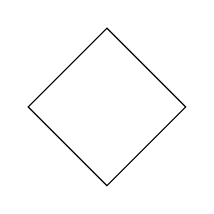
\begin{tikzpicture}
 \draw (1,0) -- (0,1) -- (-1,0) -- (0,-1) -- cycle;
\end{tikzpicture}
\end{center}
\caption{Diamond drawn using \protect\texttt{TikZ}}
\label{fig:diamond}
\end{marginfigure}


\emphasis{-,draw,begin,end,tikzpicture}
\begin{teXXX}
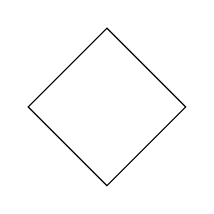
\begin{tikzpicture}
\draw (1,0) -- (0,1) -- (-1,0) -- (0,-1) -- cycle;
\end{tikzpicture}
\end{teXXX}



Sometimes it is quite useful when debugging to add a backround grid. 

\begin{marginfigure}
\begin{centering}
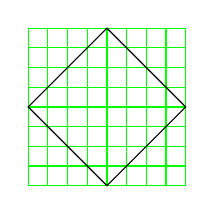
\begin{tikzpicture}
\draw[step=0.25cm,color=green] (-1,-1) grid (1,1);
\draw (1,0) -- (0,1) -- (-1,0) -- (0,-1) -- cycle;
\end{tikzpicture}
\caption{You can add a background grid using \texttt{step=0.25cm, color=green} as an option}
\end{centering}
\end{marginfigure}

\emphasis{step,color,green,grid,begin,end}
\begin{teXXX}
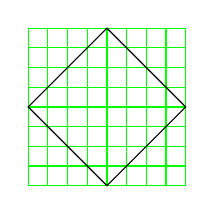
\begin{tikzpicture}
  \draw[step=0.25cm,color=green] (-1,-1) grid (1,1);
  \draw (1,0) -- (0,1) -- (-1,0) -- (0,-1) -- cycle;
\end{tikzpicture}
\end{teXXX}

The grid is specified by providing two diagonally opposing points: (-1,-1)
and (1, 1). The two options supplied give a step size for the grid lines and a
specification for the color of the grid lines, using the \docpkg{xcolor} package

\subsection{Specifying points and paths}

\begin{marginfigure}
\begin{centering}
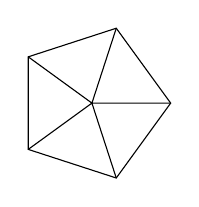
\begin{tikzpicture}
% Define the points of a regular pentagon
\path (0,0) coordinate (origin);
\path (0:1cm) coordinate (P0);
\path (1*72:1cm) coordinate (P1);
\path (2*72:1cm) coordinate (P2);
\path (3*72:1cm) coordinate (P3);
\path (4*72:1cm) coordinate (P4);
% Draw the edges of the pentagon
\draw (P0) -- (P1) -- (P2) -- (P3) -- (P4) -- cycle;
% Add "spokes"
\draw (origin) -- (P0) (origin) -- (P1) (origin) -- (P2)
(origin) -- (P3) (origin) -- (P4);
\end{tikzpicture}
\caption{Drawing a complicated polygon, using paths and the \texttt{draw} command}
\end{centering}
\end{marginfigure}


Two key ideas used in TikZ are points and paths. Both of these ideas were used
in the diamond examples. Much more is possible, however. For example, points
can be specified in any of the following ways:
\begin{enumerate}
\item  Cartesian coordinates
\item  Polar coordinates
\item  Named points
\item  Relative points
\end{enumerate}

\subsection*{coordinates}
The cartesian coordinates can be defined and named using the following syntax.

%\emphasis{begin,end,coordinate,at,draw}
%\begin{teXXX}
%\begin{tikzpicture}
%  \coordinate (A) at (0,0);
%  \coordinate (B) at (1.25,0.25);
%  \draw[blue] (A) -- (B);
%\end{tikzpicture}
%\end{teXXX}

\noindent This produces:
\begin{tikzpicture}
\coordinate (A) at (0,0);
\coordinate (B) at (1.25,0.25);
\draw[blue] (A) -- (B);
\end{tikzpicture}

%We can add labels to the points by using the |label| option.
%\begin{tikzpicture}
%\coordinate [label=left:\textcolor{orange}{$A$}] (A) at (0,0);
%\coordinate [label=right:\textcolor{orange}{$B$}]  (B) at (1.15,0.25);
%\draw[blue] (A) -- (B);
%\end{tikzpicture}
%
%\emphasis{label,left,label:,right}
%\begin{teXXX}
%\begin{tikzpicture}
%  \coordinate [label=left:\textcolor{orange}{$A$}] (A) at (0,0);
%  \coordinate [label=west:\textcolor{orange}{$B$}] (B) at (1.25,0.25);
%  \draw[blue] (A) -- (B);
%\end{tikzpicture}
%\end{teXXX}
%
%
%If you tempted to write \texttt{label=top:} it will not work, as the command accepts the following keywords.
%
%\begin{tikzpicture}
%  \coordinate [label=left:\textcolor{orange}{east}]  (A) at (0,0);
%  \coordinate [label=right:\textcolor{orange}{west}] (B) at (0,0);
%  \draw[blue] (A)--(B);
%\end{tikzpicture}
%
%
%To summarize, what we have been doing so far is to learn a set of primitive TikZ commands for drawing paths, drawing shapes and labeling them. All TikZ command work by passing options to them. For example to change the above line to an arrow, we just pass the option |->| to the |draw| command.
%
%\begin{marginfigure}[30pt]
%\begin{tikzpicture}
%  \coordinate [label=left:\textcolor{orange}{$A$}] (A) at (0,0);
%  \coordinate [label=right:\textcolor{orange}{$B$}] (B) at (1.25,0.25);
%  \draw[->,o-stealth] (A)--(B);
%\end{tikzpicture}
%\caption{Effect of the option \protect\texttt{draw[->]}.}
%\end{marginfigure}
%\emphasis{begin,end,->,draw}
%\begin{teXXX}
%\begin{tikzpicture}
%  ...
%  ...
%  \draw[->,blue] (A)--(B);
%\end{tikzpicture}
%\end{teXXX}
%
%\section*{Relative coordinates}
%\index{TikZ!coordinates, relative}
%A coordinate can be made "relative" by prefixing it with |++|. relative coordinates are useful in many applications.
%\medskip
%
%\noindent The code is simple, except before the coordinate you add the |++| signs. This tells the PGF engine to add the x,y dimensions of the new coordinate to that of its predecessor's. In many instances this is more intuitive and easier to determine.


%\begin{marginfigure}
%\begin{tikzpicture}
%\draw[step=0.5cm,color=gray] (-1,-1) grid (3.5,3);
%\draw[->,red,thick] (0,0) -- ++(1,0) -- ++(0,1) -- ++(-1,0) -- cycle;
%\draw[->,red,thick] (2,0) -- ++(1,0) -- ++(0,1) -- ++(-1,0) -- cycle;
%\draw[arrows=o-stealth,blue] (1.5,1.5) -- ++(1,0) -- ++(0,1) -- ++(-1,0) -- cycle;
%\end{tikzpicture}
%\caption{Example of use of the \protect\texttt{++} to specify relative coordinates.}
%\label{fig:relative}
%\end{marginfigure}
%\begin{teXXX}
%\begin{tikzpicture}
%  \draw[step=0.5cm,color=gray] (-1,-1) grid (3.5,3);
%  \draw[red,very thick] (0,0) -- ++(1,0) -- ++(0,1) -- ++(-1,0) -- cycle;
%  \draw[red,very thick] (2,0) -- ++(1,0) -- ++(0,1) -- ++(-1,0) -- cycle;
%  \draw[->,red,very thick] (1.5,1.5) -- ++(1,0) -- ++(0,1) -- ++(-1,0) -- cycle;
%\end{tikzpicture}
%\end{teXXX}
%
%Instead of |++| you can also use a single |+|. This also specifies a relative coordinate, but it does not "update"
%the current point for subsequent usages of relative coordinates. Thus, you can use this notation to specify
%numerous points, all relative to the same "initial" point:
%
%\begin{marginfigure}
%\begin{tikzpicture}
%\draw[step=0.5cm,color=gray] (-1,-1) grid (3.5,3);
%\draw[purple, fill=white] (0,0) -- +(1,0) -- +(1,1) -- +(0,1) -- cycle;
%\draw[purple, fill=white] (2,0) -- +(1,0) -- +(1,1) -- +(0,1) -- cycle;
%\draw[purple, fill=white] (1.5,1.5) -- +(1,0) -- +(1,1) -- +(0,1) -- cycle;
%\path (0,0) node [shape=circle,draw]{(0,0)};
%\end{tikzpicture}
%\caption{Example of use of the \protect\texttt{+} to specify relative coordinates.}
%\label{fig:relative1}
%\end{marginfigure}
%\begin{teXXX}
%  \draw (0,0) -- +(1,0) -- +(1,1) -- +(0,1) -- cycle;
%  \draw (2,0) -- +(1,0) -- +(1,1) -- +(0,1) -- cycle;
%  \draw (1.5,1.5) -- +(1,0) -- +(1,1) -- +(0,1) -- cycle;
%\end{teXXX}
%
%
%Personally, I don't favour this method of specifying co-ordinates, but it can be useful, if you are automating the production of figures through an external script\sidenote{For drawing Bezier curves, the \texttt{+} behaves differently.  You can refer to the PGF Manual for more details.}.
%
%
%\section*{Arrows}
%\index{TikZ!arrows}
%The function |->| creates a tooltip arrow. You can use different arrow tips and there is a long section for them in the PGF manual. You can even define your own.
%\begin{marginfigure}
%\centering
%\begin{tikzpicture}
%  \draw[->] (0,0) -- (2,0);
%  \draw[arrows=o-stealth,blue] (0,-0.3) -- (2,-0.3);
%  \draw[->,o-stealth,orange] (0,-0.6) -- (2,-0.6);
%  \draw[arrows=|-stealth,purple] (0,-0.9) -- (2,-0.9);
%\end{tikzpicture}
%\caption{Special arrow endings}
%\label{fig:specials}
%\end{marginfigure}
%
%\emphasis{o,stealth,begin,end,draw}
%\begin{teXXX}
%\begin{tikzpicture}
% \draw[->] (0,0) -- (2,0);
% \draw[arrows=o-stealth,blue] (0,-0.3) -- (2,-0.3);
% \draw[->,o-stealth,orange] (0,-0.6) -- (2,-0.6);
% \draw[arrows=X-stealth,purple] (0,-0.9) -- (2,-0.9);
%\end{tikzpicture}
%\end{teXXX}
%
%
%
%\begin{Verbatim}
%\begin{tikzpicture}
%% Define the points of a regular pentagon
%\path (0,0) coordinate (origin);
%\path (0:1cm) coordinate (P0);
%\path (1*72:1cm) coordinate (P1);
%\path (2*72:1cm) coordinate (P2);
%\path (3*72:1cm) coordinate (P3);
%\path (4*72:1cm) coordinate (P4);
%% Draw the edges of the pentagon
%\draw (P0) -- (P1) -- (P2) -- (P3) -- (P4) -- cycle;
%% Add "spokes"
%\draw (origin) -- (P0) (origin) -- (P1) (origin) -- (P2)
%(origin) -- (P3) (origin) -- (P4);
%\end{tikzpicture}
%\end{Verbatim}
%
%
%





\section{Nodes}
A node is a small part of a picture. When a node is created, you provide a position where the node
should be drawn and a shape. A node of shape circle will be drawn as a |circle|, a node of shape |rectangle|
as a rectangle, and so on. A node may also contain same text, which is why they can used nodes to show text.
Finally, a node can get a name for later reference.



\emphasis{node,shape,draw}
\begin{teXXX}
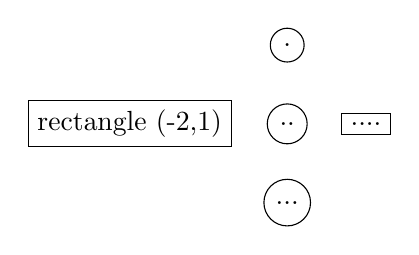
\begin{tikzpicture}
\path ( 0,2) node [shape=circle,draw] {.}
( 0,1) node [shape=circle,draw] {..}
( 0,0) node [shape=circle,draw] {...}
( 1,1) node [shape=rectangle,draw] {....}
(-2,1) node [shape=rectangle,draw] {rectangle (-2,1)};
\end{tikzpicture}
\end{teXXX}
\medskip

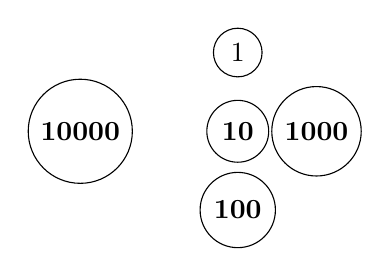
\begin{tikzpicture}
\path ( 0,2) node [shape=circle,draw] {1}
( 0,1) node [shape=circle,draw] {\textbf{10}}
( 0,0) node [shape=circle,draw] {\textbf{100}}
( 1,1) node [shape=circle,draw] {\textbf{1000}}
(-2,1) node [shape=circle,draw] {\textbf{10000}};
\end{tikzpicture}

In the above code, this text is empty (because of the
|empty {}|). So, why do we see anything at all at all the nodes? The answer is the draw option for the node operation: It
causes the |shape| around the text" to be drawn. If you have an empty |{}|, PGF still sees the empty space as a character and justs draws around it. The reason is than TikZ automatically adds some space around the text. The amount is set
using the option inner sep. So, to increase the size of the nodes. Modifying the example slightly we get.



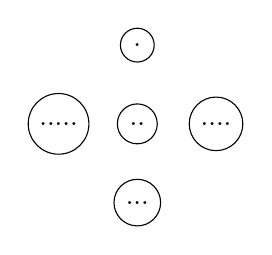
\begin{tikzpicture}
\path ( 0,2) node [shape=circle,draw] {.}
( 0,1) node [shape=circle,draw] {..}
( 0,0) node [shape=circle,draw] {...}
( 1,1) node [shape=circle,draw] {....}
(-1,1) node [shape=circle,draw] {.....};
\end{tikzpicture}

\noindent As you can observe the size of the circle has been adjusted to fit the text that is enclosing it.

\subsection{Drawing circles}

\begin{marginfigure}
\begin{centering}
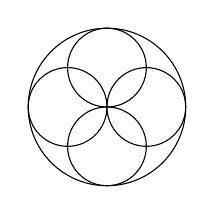
\begin{tikzpicture}
\draw (0,0) circle (1cm);
\draw (0.5,0) circle (0.5cm);
\draw (0,0.5) circle (0.5cm);
\draw (-0.5,0) circle (0.5cm);
\draw (0,-0.5) circle (0.5cm);
\end{tikzpicture}
\caption{Drawing multiple circles, using mutiple \texttt{draw} commands}
\end{centering}
\end{marginfigure}


A circle is specified by providing its center point and the desired radius. The
command:

\medskip

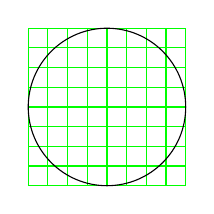
\begin{tikzpicture}
  \draw[step=0.25cm,color=green] (-1,-1) grid (1,1);
  \draw (0,0) circle (1cm);
\end{tikzpicture}
\medskip

\begin{teXXX}
\begin{tikzpicture}
  \draw (x,y) circle (dia);
\end{tikzpicture}
\end{teXXX}



You  can use one |\draw| command to draw multiple circles as shown in \fref{fig:circles}


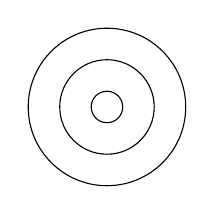
\begin{tikzpicture} 
 \draw (0,0) 
  circle (1cm)
  circle (0.6cm)
  circle (0.2cm)
 ;
\end{tikzpicture}

\emphasis{circle,begin,end}
\begin{teXXX}
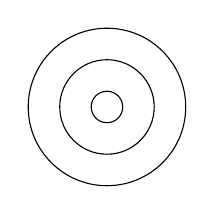
\begin{tikzpicture} 
 \draw (0,0) 
  circle (1cm)
  circle (0.6cm)
  circle (0.2cm)
 ;
\end{tikzpicture}
\end{teXXX}




\begin{marginfigure}
\begin{center}
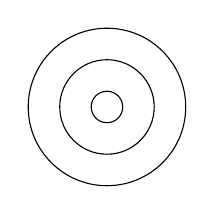
\begin{tikzpicture}
\draw (0,0) circle (1cm)
circle (0.6cm)
circle (0.2cm);
\end{tikzpicture}
\caption{You can use one draw command to draw multiple circles}
\label{fig:circles}
\end{center}
\caption{Drawing multiple circles, using mutiple \texttt{circle} commands}
\end{marginfigure}

\subsection{Drawing ellipses}

Ellipses can be drawn in a similar fashion to circles. As an ellipse needs two center points to be specified the command used has the following general form:

\begin{verbatim}
\draw (a,b) ellipse (r1 dim and r2 dim);
\end{verbatim}

We can draw two ellipses as shown in the figure, using the code:
\begin{teX}
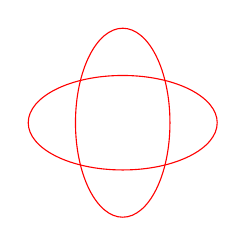
\begin{tikzpicture}[scale=0.6]
\draw[color=red] (0,0) ellipse (2cm and 1cm);
\draw[color=red] (0,0) ellipse (1cm and 2cm);
\end{tikzpicture}
\end{teX}
\begin{marginfigure}
\begin{centering}
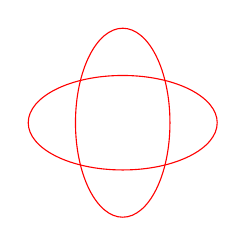
\begin{tikzpicture}[scale=0.6]
\draw[color=red] (0,0) ellipse (2cm and 1cm);
\draw[color=red] (0,0) ellipse (1cm and 2cm);
\end{tikzpicture}
\caption[Drawing ellipses]{Use the draw command in combination with ellipse to draw ellipses}
\end{centering}
\end{marginfigure}

\begin{teX}
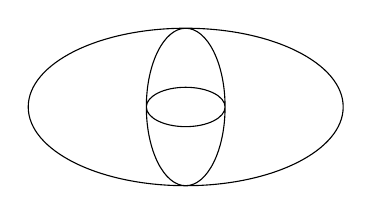
\begin{tikzpicture}
\draw (0,0) ellipse (2cm and 1cm)
ellipse (0.5cm and 1 cm)
ellipse (0.5cm and 0.25cm);
\end{tikzpicture}
\caption{Drawing multiple circles, using mutiple \texttt{draw} commands}
\end{teX}

\section{Drawing more complicated shapes}

\begin{marginfigure}
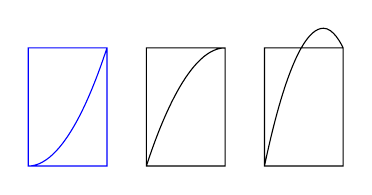
\begin{tikzpicture}
\draw[color=blue] (0,0) rectangle (1,1.5)
(0,0) parabola[color=orange] (1,1.5);
\draw[xshift=1.5cm] (0,0) rectangle (1,1.5)
(0,0) parabola[bend at end] (1,1.5);
\draw[xshift=3cm] (0,0) rectangle (1,1.5)
(0,0) parabola bend (.75,1.75) (1,1.5);
\end{tikzpicture}
\caption{Parabolas drawn using the parabola command}
\label{fig:parabola}
\end{marginfigure}

we can place a parabola in a rectangle as shown in \fref{fig:parabola}, by using the |rectangle| and the |parabola| options.

\subsection*{The shape library}

\begin{tikzpicture}
\draw [help lines] (0,0) grid (2,2);
\draw [blue, dashed] (1,1) circle(1cm);
\draw [red, dashed] (1,1) circle(.5cm);
\node [star, star point height=.5cm, minimum size=2cm, draw]
at (1,1) {S};
\end{tikzpicture}

\section{Iterations}
One convenient construct provided with TikZ is a |foreach| command sequence
\begin{marginfigure}
\begin{centering}
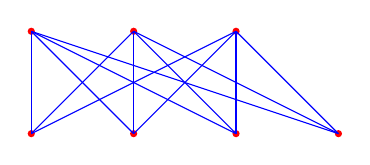
\begin{tikzpicture}[scale=1.3, color=red]
\foreach \i in {1,...,4}
{
  \path (\i,0) coordinate (X\i);
  \fill (X\i) circle (1pt);
}
  \foreach \j in {1,...,3}
{
  \path (\j,1) coordinate (Y\j);
  \fill (Y\j) circle (1pt);
}
\foreach \i in {1,...,4}
{
  \foreach \j in {1,...,3}
  {
     \draw[color=blue] (X\i) -- (Y\j);
  }
}
\end{tikzpicture}
\caption{Drawing a bi-partite garph using foreach loops}
\end{centering}
\end{marginfigure}

\begin{lstlisting}[language={[common]TeX},% 
                           alsolanguage={[LaTeX]TeX},% 
                           alsolanguage={[primitive]TeX},%
                           alsolanguage={Verse}]
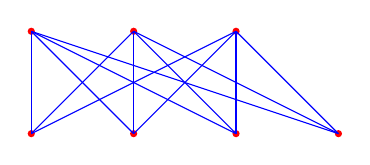
\begin{tikzpicture}[scale=1.3, color=red]
\foreach \i in {1,...,4}
{
  \path (\i,0) coordinate (X\i);
  \fill (X\i) circle (1pt);
}
  \foreach \j in {1,...,3}
{
  \path (\j,1) coordinate (Y\j);
  \fill (Y\j) circle (1pt);
}
\foreach \i in {1,...,4}
{
  \foreach \j in {1,...,3}
  {
     \draw[color=blue] (X\i) -- (Y\j);
  }
}
\end{tikzpicture}
\end{lstlisting}



\begin{marginfigure}
% Define styles for the different kind of edges in a Feynman diagram
\tikzset{
    photon/.style={decorate, decoration={snake}, draw=red},
    electron/.style={draw=blue, postaction={decorate},
        decoration={markings,mark=at position .55 with {\arrow[draw=blue]{>}}}},
    gluon/.style={decorate, draw=magenta,
        decoration={coil,amplitude=4pt, segment length=5pt}} 
}

\begin{tikzpicture}[
        thick,
        % Set the overall layout of the tree
        level/.style={level distance=1.5cm},
        level 2/.style={sibling distance=2.6cm},
        level 3/.style={sibling distance=2cm},
        scale=0.5
        ]
    \coordinate
        child[grow=left]{
            child {
                node {$g$}
                % The 'edge from parent' is actually not needed because it is
                % implicitly added.
                edge from parent [gluon]
            }
            child {
                node {$g$}
                edge from parent [gluon]
            }
            edge from parent [gluon] node [above=3pt] {$g$}
        }
        % I have to insert a dummy child to get the tree to grow
        % correctly to the right.
        child[grow=right, level distance=0pt] {
        child  {
            child {
                child {
                    node {$\bar{d}$}
                    edge from parent [electron]
                }
                child {
                    node {$u$}
                    edge from parent [electron]
                }
                edge from parent [photon]
            }
            child {
                node {$b$}
                edge from parent [electron]
            }
            edge from parent [electron]
            node [below] {$t$}
        }
        child {
            child {
                node {$\bar{b}$}
                edge from parent [electron]
            }
            child {
                child {
                    node {$\bar{v}$}
                    edge from parent [electron]
                }
                child {
                    node {$e^{-}$}
                    edge from parent [electron]
                }
                edge from parent [photon]
            }
            edge from parent [electron]
            node [above] {$\bar{t}$}
        }
    };
\end{tikzpicture}
\caption{Feynman diagrams}
\end{marginfigure}




\subsection{Loading data from files}
Scientific work, especially that associated with research sometimes generate
a lot of data. The data would normally come from external applications and stored in files. With |TikZ| one can import the data
by using the word |file|:

\emphasis{addplot,file,x}
\begin{teXXX}
 \addplot file {./raw/wavefunctions/wavefunc\x.dat};
\end{teXXX}

In the example we use a file with a path. The data is saved in
files with the same name but a different ending. We use a |foreach| function to add the ending i.e, the file names are |wavefunc1|, |wavefunc2| and |wavefunc3|. By using external data files and the foreach command it can substantially reduce the amount of text in the macros. This improves debugging and readability.

\begin{marginfigure}
\begin{tikzpicture}[scale=0.6]
    \begin{axis}[
    xlabel=$n$,
    ylabel=$\Theta{j}{n}$]
    \foreach \x in {0,...,2}
    {
        \addplot file {./raw/wavefunctions/wavefunc\x.dat};
    }
    \legend{$j=0$,$j=1$,$j=2$};
    \end{axis}
\end{tikzpicture}
\caption{Example plot with data imported from external files, using \texttt{file}}
\end{marginfigure}


\begin{teXXX}
\begin{tikzpicture}[scale=0.6]
  \begin{axis}[
    xlabel=$n$,
    ylabel=$\Theta{j}{n}$]
    \foreach \x in {0,...,2}
    {
      \addplot file {./raw/wavefunctions/wavefunc\x.dat};
    }
    \legend{$j=0$,$j=1$,$j=2$};
  \end{axis}
\end{tikzpicture}
\end{teXXX}



\section*{Plotting functions}
Functions can be defined for plotting using a variety of methods. They are powerful but generally different to remember.

\begin{marginfigure}
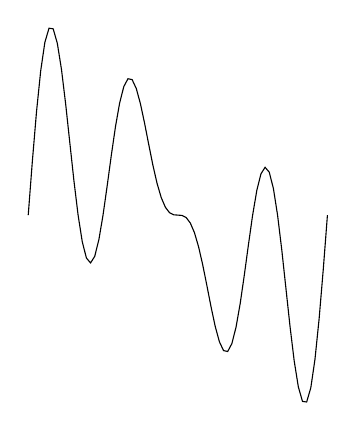
\begin{tikzpicture}[x=3.8cm/360]
  \pgfplothandlerlineto
  \pgfplotfunction{\x}{0,5,...,360}{\pgfpointxy{\x}{sin(\x)+sin(3*\x)+sin(4*\x)}}
  \pgfusepath{stroke}
\end{tikzpicture}
\end{marginfigure}

\emphasis{begin,end,pgfplothandlerlineto,pgfplotfunction,pgfusepath,x,pgfpointxy}
\begin{teXXX}
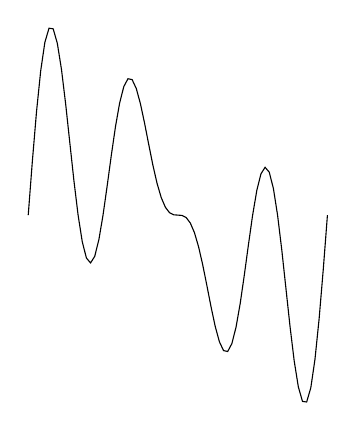
\begin{tikzpicture}[x=3.8cm/360]
  \pgfplothandlerlineto
  \pgfplotfunction{\x}{0,5,...,360}{\pgfpointxy{\x}{sin(\x)
                      +sin(3*\x)+sin(4*\x)}}
  \pgfusepath{stroke}
\end{tikzpicture}
\end{teXXX}

\begin{marginfigure}
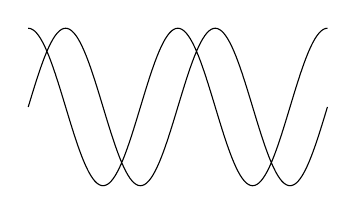
\begin{tikzpicture}[x=3.8cm/720]
  \pgfplothandlerlineto
  \pgfplotfunction{\x}{0,5,...,720}{\pgfpointxy{\x}{sin(\x)}}
  \pgfplotfunction{\x}{0,5,...,720}{\pgfpointxy{\x}{cos(\x)}} 
  \pgfusepath{stroke}
\end{tikzpicture}
\end{marginfigure}

\newpage

\section{Saving Data to a file}

You can save your data to a file in many ways. One easy way is to use
the \docpkg{filecontents} package. This package extends the LaTeX environment
with the same name, but allows you to overwrite the file {\protect\ctan{filecontents}}.

\begin{teXXX}
\documentclass[justified]{tufte-book}
\usepackage{pgfplots,lipsum,booktabs}
\usepackage{pgfplotstable}
\pgfplotsset{compat=newest}
\usepackage{filecontents*}
\begin{filecontents}{my1.dat}
    Label       value       num
    Integrity     33         4
    Standalone    14         3
    Interface      6         2
    Overall       18         1
\end{filecontents*}
\begin{document}
    your code here ...
\end{document}
\end{teXXX}

It is good practice to keep, such data at the top of your file, although with
the |filecontents| package, they can be inserted anywhere. Sometimes it maybe
easier to have a number of minimal files with the type of charts you using regularly and just update the data on top. In general if the data is entered
by hand rather than generated automatically by software this is a good way
to keep your work tidy.

\newenvironment{Chart}[1][black!70!green]{%
%%  defaults
    \gdef\level##1{Level ##1}
    \def\setchartwidth##1{%
      \def\chartwidth{##1}}%
    \setchartwidth{3.9cm}%
    \def\chartcolor{#1}
    \newcommand\addTitle[2][test]{
%% For the chart title we set it in a minipage for
%% better control
    \def\charttitle{\minipage{4cm}%
       \footnotesize %
       \centering\textbf{##2}\\##1%
       \endminipage}}%
   \def\xlabel{Completion (\%)}%
%% renders the chart 
    \def\renderChart{%
%%
    \footnotesize%
%%
%%
    \IfFileExists{#1.dat}{Test}{}
   \begin{tikzpicture}
   \begin{axis}[
    xbar, width=\chartwidth,title=\charttitle,
    y=0.5cm, enlarge y limits={true, abs value=0.75},
    xmin=0, xmax=100,enlarge x limits={upper, value=0.25},
    xlabel=\xlabel,
    %ylabel=Label,
    xmajorgrids=true,
    ytick=data,
    yticklabels from table={\dataTable}{Label},
    nodes near coords, nodes near coords align=horizontal
     ]
    \addplot[draw=none, fill=\chartcolor] table [x=value, y=num]
    {\dataTable};
    \end{axis}%
    \end{tikzpicture}}}
{}

\begin{figure*}
\centering

\hskip-2cm\begin{Chart}
 \addTitle[Mechanical Systems]{Shangri-la}
 \def\dataTable{SH-mechanical.dat}
 \renderChart
\end{Chart}\hspace{0.3cm}
\begin{Chart}
 \addTitle[FM-200 System]{All areas}
 \def\dataTable{my1.dat}
 \renderChart
\end{Chart}
\begin{Chart}
 \addTitle[Electrical Works]{Merweb}
 \def\dataTable{my6.dat}
 \renderChart
\end{Chart}
\caption{Mechanical Systems Shangrila. Commissioning status}
\end{figure*}

\begin{filecontents*}{my1.dat}
Label     value       num
Integrity         33            4
Standalone      14            3
Interface        6            2
Overall           18            1
\end{filecontents*}

\begin{filecontents*}{SH-mechanical.dat}
Label     value       num
{Fan coil units}       43             8
{Air Handling Units}       13             7 
{CW Pumps}       13             6
{ECU}       11             5
{Pressurization Fans}        15             4
{Smoke Extract Fan}       5             3
{Jet fan}       5             2
{Overall}       12              1
\end{filecontents*}

\begin{filecontents*}{my6.dat}
Label    value         num   other
{Level 7}  50           11   13
L6         90           10   12
L5       80             9    16
L4       90             8    18
L3       70             7    90
L2       80             6    21
L1       70             5    22
\end{filecontents*}

\begin{filecontents*}{carparkventilation.dat}
Label    value         num   other
L5         50           11   13
L4         90           10   12
L3         80           9    16
GR         90           8    18
B1         70           7    90
B2         80           6    21
B3         70           5    22
\end{filecontents*}
%% CO SYSTEM
%% DATA
\begin{filecontents*}{carparkco.dat}
Label    value         num   other
L5         78           7   13
L4         90           6   12
L3         80           5    16
GR         90           4    18
B1         70           3    90
B2         80           2    21
B3         70           1    22
B5         50          {}    {}
\end{filecontents*}

\begin{filecontents*}{carparkco2.dat}
value,   num,   other,
78,       7,   13,
90,       6,   12,
80,       5,    16,
90,       4,    18,
70,       3,    90,
80,       2,    21,
70,       1,    22,
\end{filecontents*}






















